\documentclass{article}
\usepackage[utf8]{inputenc}
\usepackage[T1]{fontenc} % uses T1 fonts (better quality)
\usepackage{lmodern} % uses Latin Modern fonts
\usepackage[table,xcdraw,dvipsnames]{xcolor}
\usepackage[margin=1in]{geometry}
\usepackage{nopageno} % no page numbers
\usepackage{graphicx}
\graphicspath{ {./graphics/} }
\usepackage{bm}
\usepackage{caption}
\usepackage{minted} % code syntax
\usemintedstyle{vs}

\title{}
\begin{document}
% \begin{titlepage}
% \vspace*{\fill}
 	\begin{center}
     \line(1,0){300}\\[0.25cm]
 	\large{\bfseries Homework 3}\\
 	\textsc{\large David Kirby}\\
 	\textsc{\large Due: 12 May 2020}\\
 	\line(1,0){300}\\[0.75cm]
 	\end{center}
 %	\vfill
% \end{titlepage}

\begin{enumerate}
\item \textbf{(15 points)} For the following problem, assume a 5-stage pipelined processor with forwarding and hardware interlocking. Also, assume branch resolution is in the Execute stage. Consider the code below:\begin{verbatim}
    addi $t2, $t1, 60
loop:
    lw $t4, 0($t1)
    lw $t5, 4($t1)
    xor $t6, $t4, $t5
    sw $t6, 8($t1)
    addi $t1, $t1, 12
    bne $t1, $t2, loop
    \end{verbatim}\par
\begin{enumerate}
    \item How many loop iterations does the above code execute?\par
    \textbf{The code above will branch back to the loop as long as \texttt{\$t1}$\bm\ne$\texttt{\$t2}. This means there will be five loop iterations since \texttt{\$t1} will increment by 12 each loop until it reaches 60, at which point it will no longer satisfy the \texttt{bne} causing a branch not taken situation and move on to the next instructions (if there are any).}
    \item Identify the data dependencies in the above code.
        \begin{figure}[h!]
        \centering
        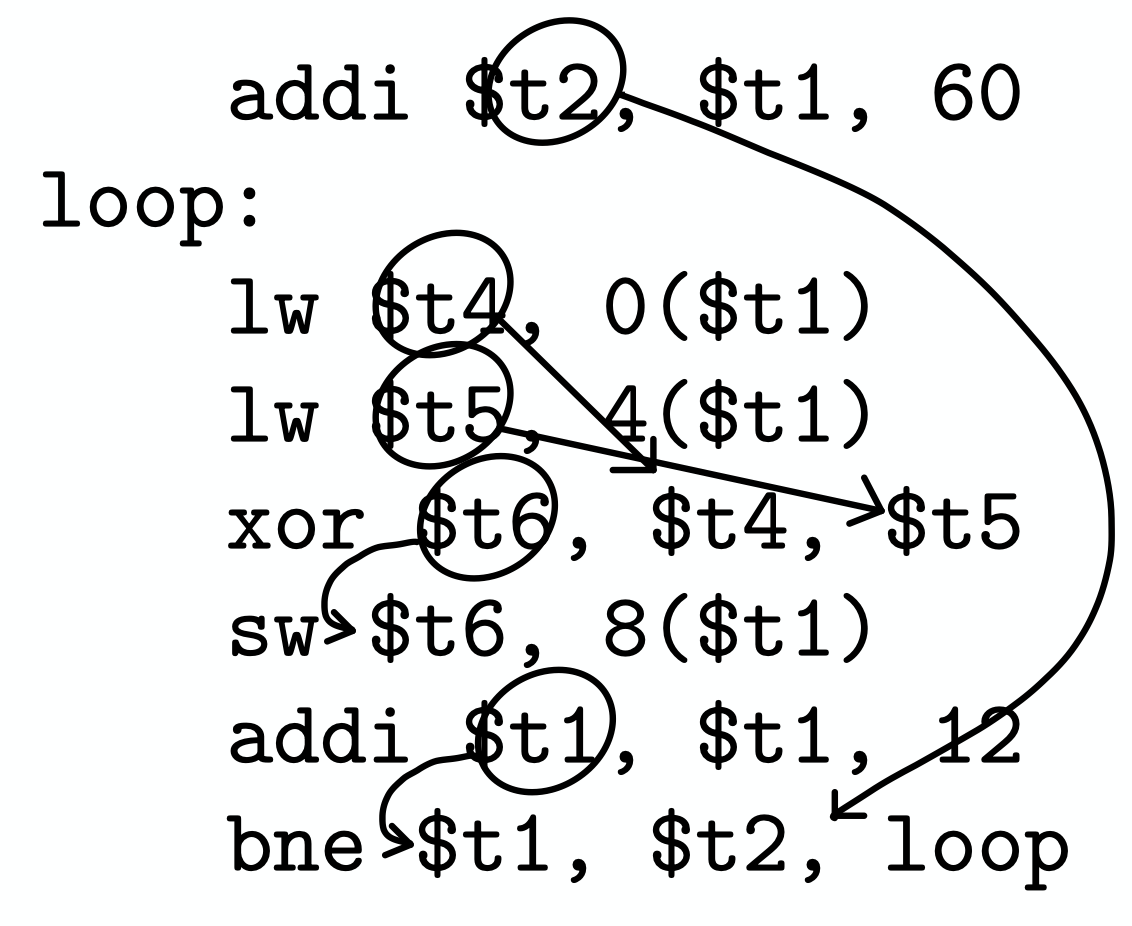
\includegraphics[width=0.25\textwidth]{Screen Shot 2020-05-06 at 16.05.44.png}
        % \caption{}
        % \label{fig:I2Cdemo}
        \end{figure}
    \item Draw the pipeline execution diagram for the first two iterations of the above code when an “assume not taken” branching scheme without a branch delay slot is used.\par
        \begin{figure}[h!]
        \centering
        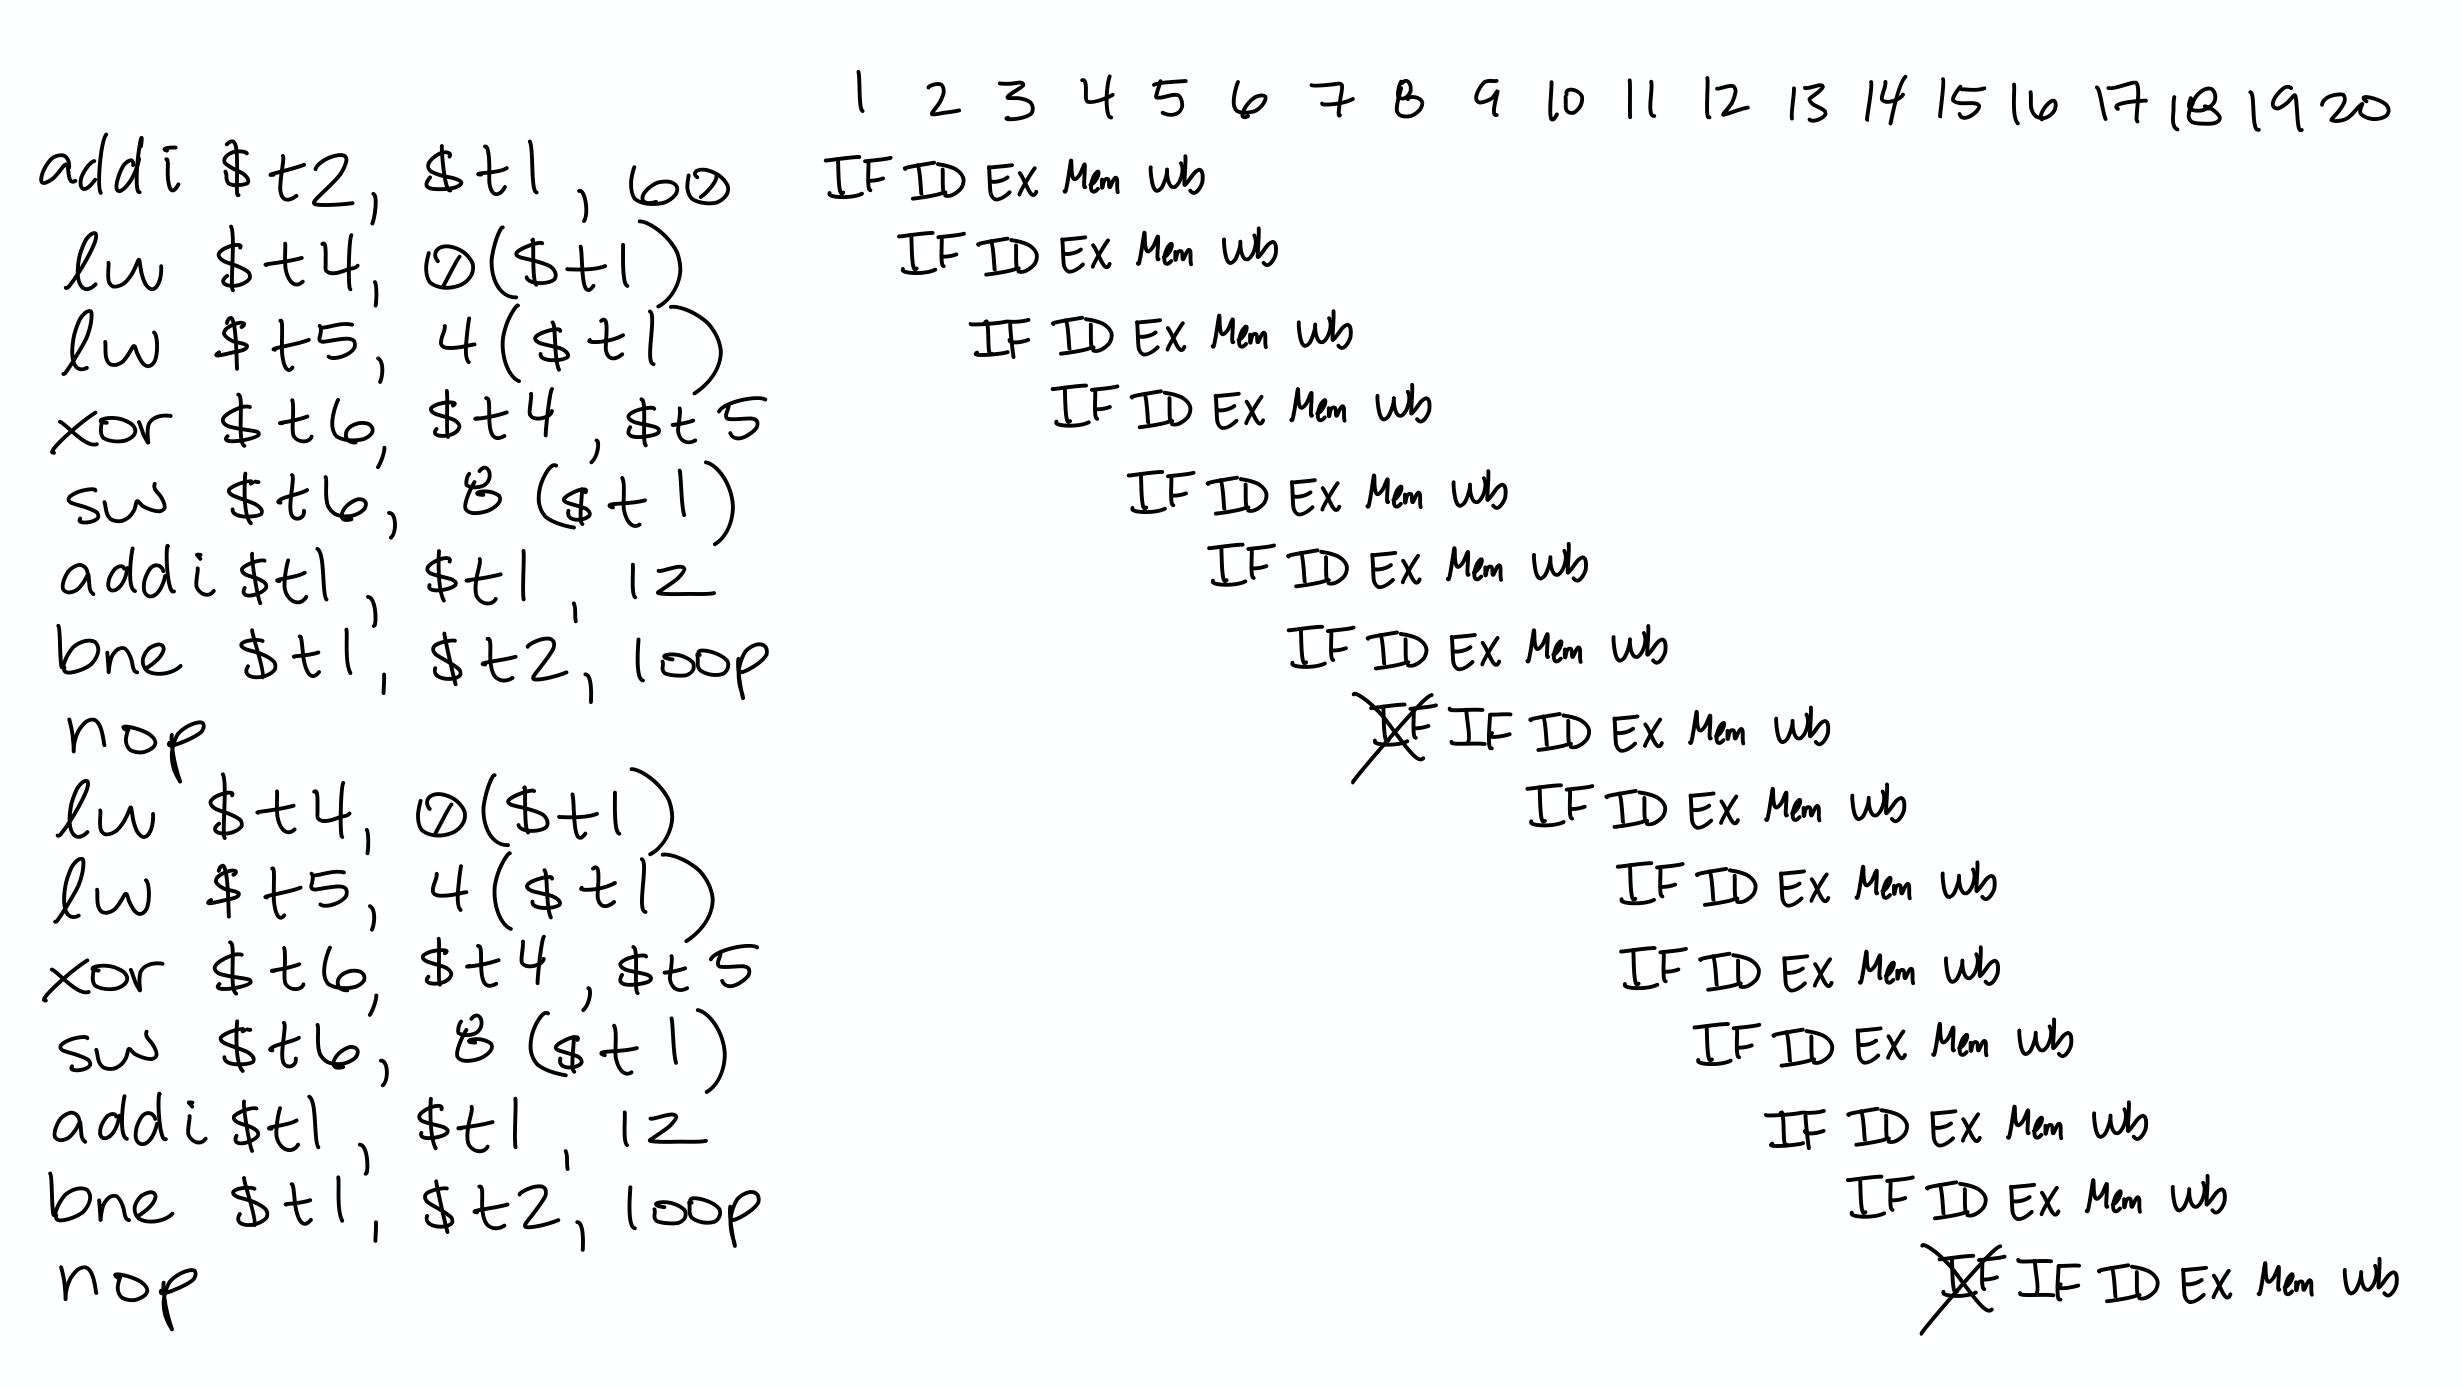
\includegraphics[width=0.55\textwidth]{q1-c.png}
        % \caption{}
        % \label{fig:I2Cdemo}
        \end{figure}
    \item How many clock cycles are required to execute the above code to completion when an “assume not taken” branching scheme without a branch delay slot is used?\par
    \textbf{Without a branch delay slot, 20 clock cycles.}
    \item Modify the code to take advantage of a branch delay slot. How many clock cycles are required to executed your modified code to completion when an “assume not taken” branching scheme with a branch delay slot is used?\par
    \textbf{With branch delay slots, 17 clock cycles.}
        \begin{figure}[h!]
        \centering
        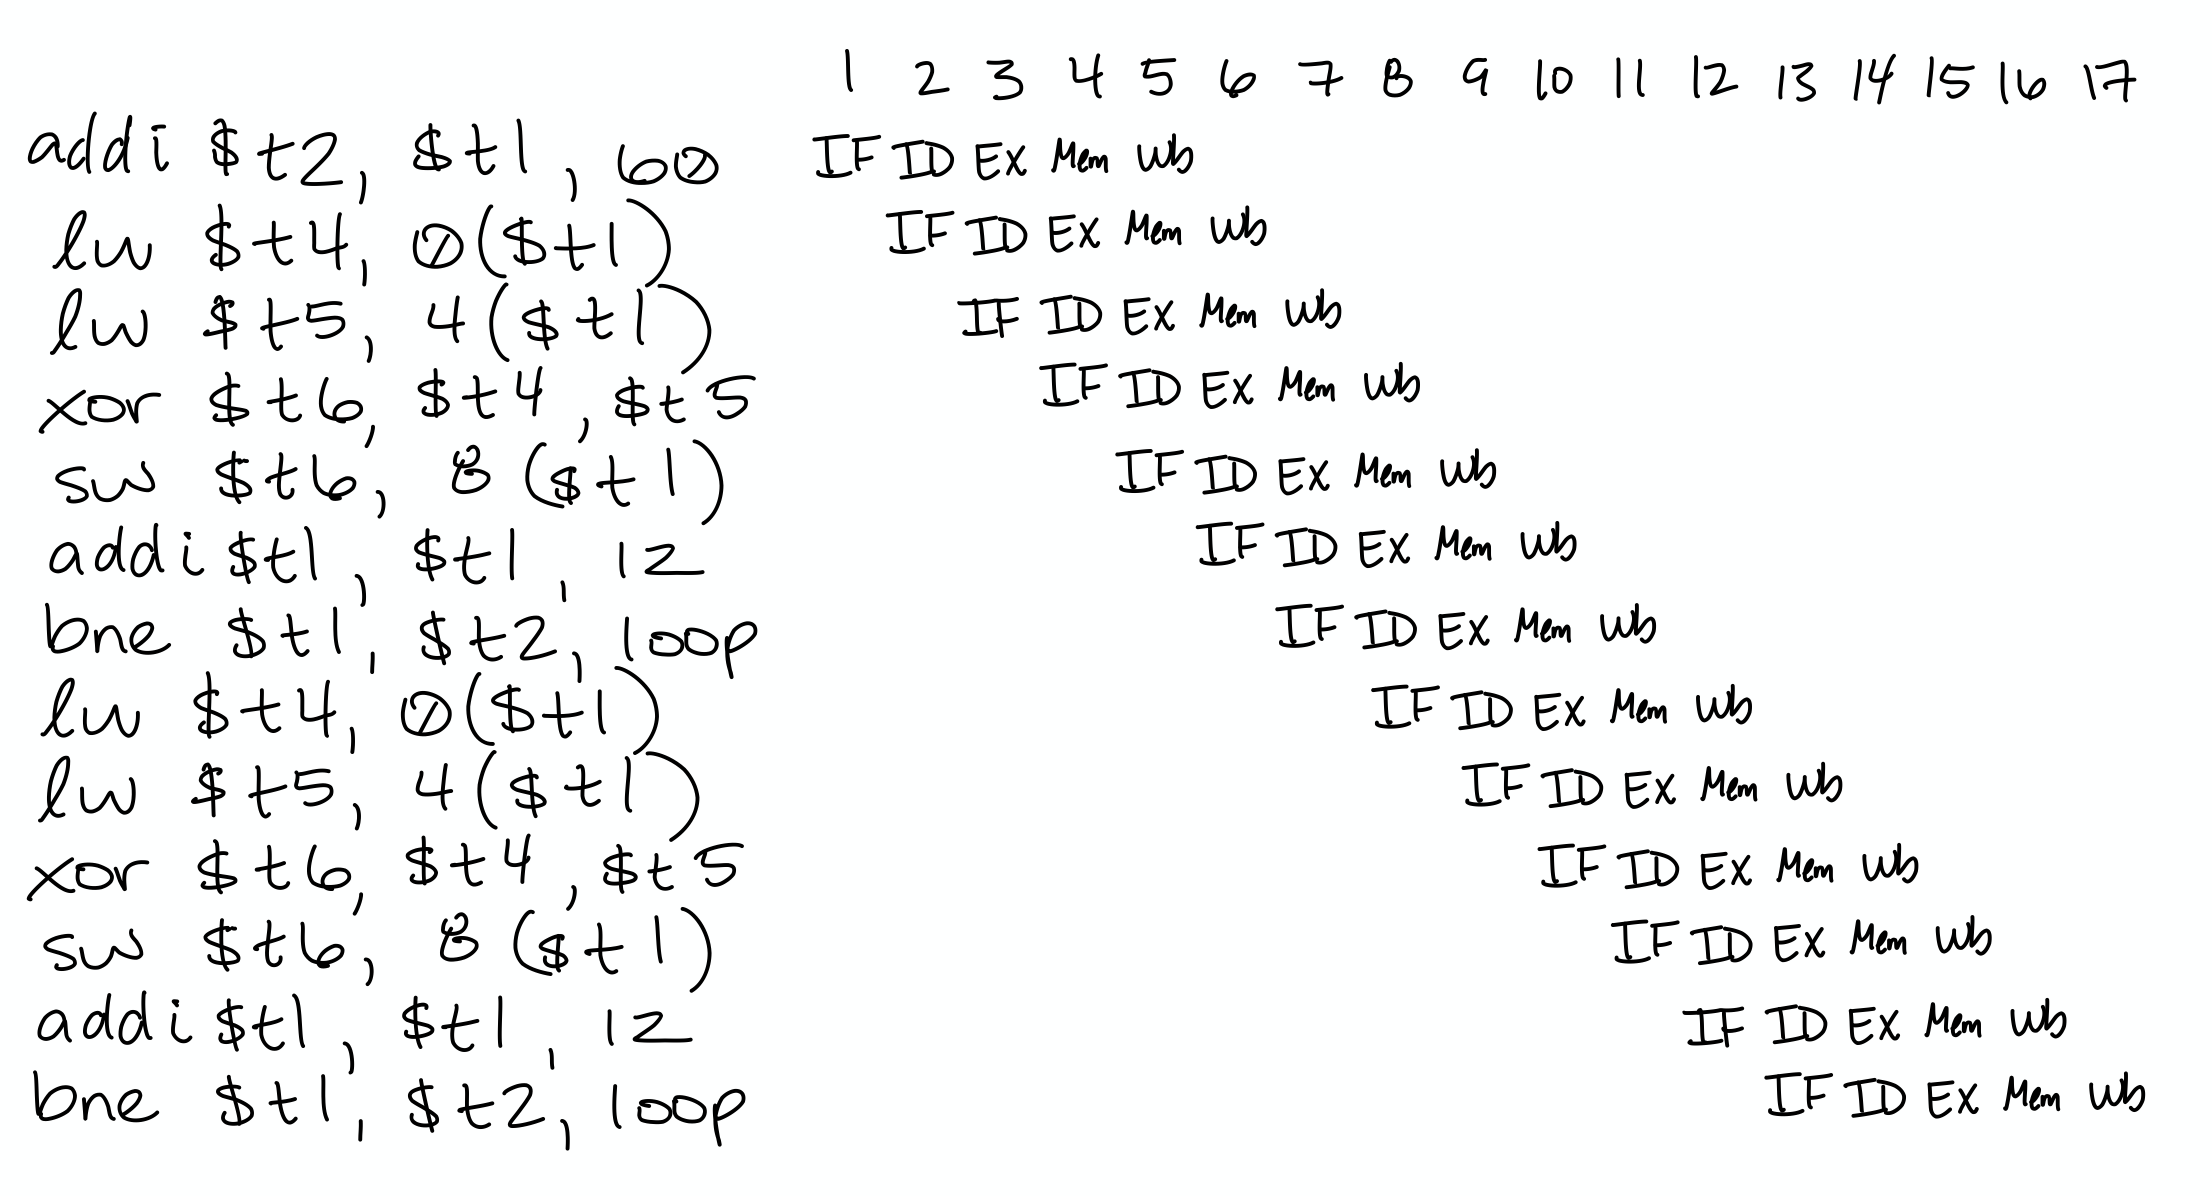
\includegraphics[width=0.55\textwidth]{q1-d.png}
        % \caption{}
        % \label{fig:I2Cdemo}
        \end{figure}
    \item How many clock cycles are required to execute you modified code assuming a 100\% correct branch predictor in the decode stage in addition to the branch delay slot.\par
    \textbf{Still 17 clock cycles.}
        \begin{figure}[h!]
        \centering
        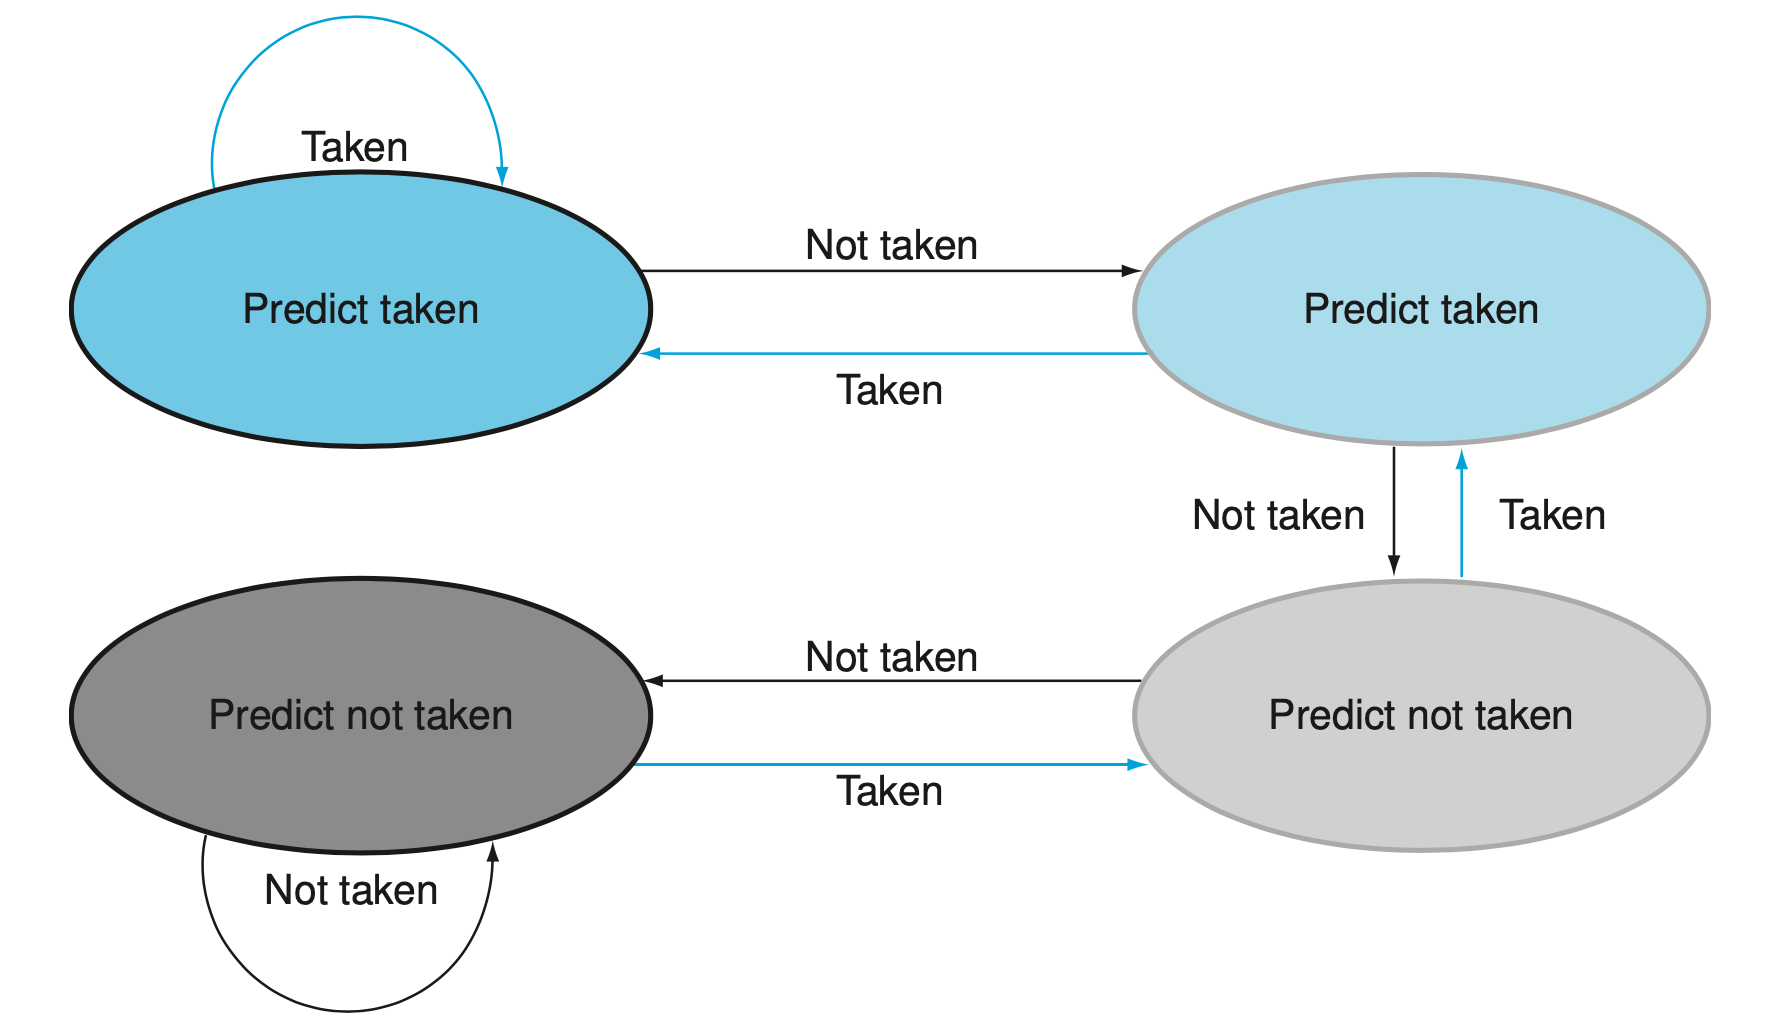
\includegraphics[width=0.50\textwidth]{Screen Shot 2020-05-06 at 16.14.46.png}
        % \caption{}
        % \label{fig:I2Cdemo}
        \end{figure}
    \item Consider the use of the two-bit predictor shown above in the decode stage. Assuming the predictor starts in the top right state, how many clock cycles are required to execute your code?\par
    \textbf{15 clock cycles}
    \item What is the accuracy of this predictor given the code above? Compare that to the accuracy of the “assume not taken” scheme.\par
    \textbf{100\%}
    \item What speedup does the branch predictor from Problem \fcolorbox{red}{white}{1g} provide over the “assume not taken” scheme from Problem \fcolorbox{red}{white}{1d}?\par
    \textbf{$\bm{\frac{15}{17}= }$12\% speedup}
    \item Further rearrange the code to reduce the number of stalls due to data dependencies.\par
    \textbf{}
\end{enumerate}
\newpage\item \textbf{(30 points)} The following problems are related to techniques and terminology of the memory hierarchy.
\begin{enumerate}
    \item Define spacial and temporal locality. Describe the role spacial and temporal locality play in the memory hierarchy.\par
    \textbf{Spatial locality states that if a data location is referenced, there is a high likelihood that nearby locations will be referenced as well. Temporal locality deals with time and states that if a data location is referenced, there is a high likelihood that it will be referenced again. Instruction cache uses lots of spatial and temporal locality compared to data access cache and helps to speed up memory hierarchy.}
    \item Define and briefly describe the types of cache misses talked about in lecture. Remember the three C’s.\par
    \textbf{Cache misses can be divided into compulsory (empty cache), capacity (cache size is too small), or conflict (cache is not fully associative).}
    \item Draw the hardware diagram of a \textit{direct-mapped cache}. Be sure to label the various portions of the address.\par
    \textbf{The numbers above each cache bit shown below are the cache index, which map the cache to the main memory.}
\begin{table}[ht]
\centering
\caption*{Cache}
\begin{tabular}{llllllll}
\multicolumn{1}{c}{\rotatebox[origin=c]{90}{\ \fcolorbox{white}{white}{000}}} & \multicolumn{1}{c}{\rotatebox[origin=c]{90}{\ \fcolorbox{Gray}{white}{001}}}                       & \multicolumn{1}{c}{\rotatebox[origin=c]{90}{\ \fcolorbox{white}{white}{010}}} & \multicolumn{1}{c}{\rotatebox[origin=c]{90}{\ \fcolorbox{white}{white}{011}}} & \multicolumn{1}{c}{\rotatebox[origin=c]{90}{\ \fcolorbox{white}{white}{100}}} & \multicolumn{1}{c}{\rotatebox[origin=c]{90}{\ \fcolorbox{RoyalBlue}{white}{101}}}                       & \multicolumn{1}{c}{\rotatebox[origin=c]{90}{\ \fcolorbox{white}{white}{110}}} & \multicolumn{1}{c}{\rotatebox[origin=c]{90}{\ \fcolorbox{white}{white}{111}}} \\ \hline
\multicolumn{1}{|l|}{}  & \multicolumn{1}{l|}{\cellcolor{Gray}} & \multicolumn{1}{l|}{}   & \multicolumn{1}{l|}{}   & \multicolumn{1}{l|}{}   & \multicolumn{1}{l|}{\cellcolor{RoyalBlue}} & \multicolumn{1}{l|}{}   & \multicolumn{1}{l|}{}   \\ \hline
\end{tabular}
\end{table}
\vspace{3cm}
\begin{table}[ht]
\centering
\begin{tabular}{llllllllllllllllllllllllllllllll}
\hline
\multicolumn{1}{|l|}{} & \multicolumn{1}{l|}{\cellcolor{Gray}} & \multicolumn{1}{l|}{} & \multicolumn{1}{l|}{} & \multicolumn{1}{l|}{} & \multicolumn{1}{l|}{\cellcolor{RoyalBlue}} & \multicolumn{1}{l|}{} & \multicolumn{1}{l|}{} & \multicolumn{1}{l|}{} & \multicolumn{1}{l|}{\cellcolor{Gray}} & \multicolumn{1}{l|}{} & \multicolumn{1}{l|}{} & \multicolumn{1}{l|}{} & \multicolumn{1}{l|}{\cellcolor{RoyalBlue}} & \multicolumn{1}{l|}{} & \multicolumn{1}{l|}{} & \multicolumn{1}{l|}{} & \multicolumn{1}{l|}{\cellcolor{Gray}} & \multicolumn{1}{l|}{} & \multicolumn{1}{l|}{} & \multicolumn{1}{l|}{} & \multicolumn{1}{l|}{\cellcolor{RoyalBlue}} & \multicolumn{1}{l|}{} & \multicolumn{1}{l|}{} & \multicolumn{1}{l|}{} & \multicolumn{1}{l|}{\cellcolor{Gray}} & \multicolumn{1}{l|}{} & \multicolumn{1}{l|}{} & \multicolumn{1}{l|}{} & \multicolumn{1}{l|}{\cellcolor{RoyalBlue}} & \multicolumn{1}{l|}{} & \multicolumn{1}{l|}{} \\ \hline
\multicolumn{3}{c}{\rotatebox[origin=c]{90}{00\fcolorbox{Gray}{white}{001}\ }}                                                                      & \multicolumn{1}{c}{}  & \multicolumn{3}{c}{\rotatebox[origin=c]{90}{00\fcolorbox{RoyalBlue}{white}{101}\ }}                                                                     & \multicolumn{1}{c}{}  & \multicolumn{3}{c}{\rotatebox[origin=c]{90}{01\fcolorbox{Gray}{white}{001}\ }}                                                                     & \multicolumn{1}{c}{}  & \multicolumn{3}{c}{\rotatebox[origin=c]{90}{01\fcolorbox{RoyalBlue}{white}{101}\ }}                                                                     & \multicolumn{1}{c}{}  & \multicolumn{3}{c}{\rotatebox[origin=c]{90}{10\fcolorbox{Gray}{white}{001}\ }}                                                                     & \multicolumn{1}{c}{}  & \multicolumn{3}{c}{\rotatebox[origin=c]{90}{10\fcolorbox{RoyalBlue}{white}{101}\ }}                                                                     & \multicolumn{1}{c}{}  & \multicolumn{3}{c}{\rotatebox[origin=c]{90}{11\fcolorbox{Gray}{white}{001}\ }}                                                                     & \multicolumn{1}{c}{}  & \multicolumn{3}{c}{\rotatebox[origin=c]{90}{11\fcolorbox{RoyalBlue}{white}{101}\ }}                                                                     & \multicolumn{1}{c}{}
\end{tabular}
\caption*{Main Memory}
\end{table}
    \item Compare and contrast \textit{write-back} and \textit{write-through} cache write policies. When might one be preferred over the other?\par
    \textbf{There are two different strategies for handling writes:
    \begin{enumerate}
        \item \textit{Write-through}: in which we always write data to the next level in hierarchy. \textit{Write-through} is simple to implement and keeps the next level of memory consistent, but is a major performance bottleneck because the processor must stall on multiple writes and creates congestion on the bus and next level of memory.\\
        \item \textit{Write-back}: Only writes data to the next level during a block replacement. \textit{Write-back} provides much better performance as writes do not go to the next level until the block is being evicted. This significantly reduces congestion on the bus and next level of memory; however, this comes at the cost of complexity.
    \end{enumerate}}
    \item Compare and contrast \textit{write-allocate} and \textit{no write-allocate}. When might one be preferred over the other? Can either of these schemes be used with \textit{write-back} and \textit{write-through}? Why or why not?\par
    \textbf{In addition to \textit{write-back} vs. \textit{write-through}, we must choose between \textit{write-allocate} and \textit{no write-allocate}. What these two strategies define is what the cache does in the case of a write to a block of memory that is not already in the cache.
    \begin{enumerate}
        \item \textit{Write-allocate}: Write-misses force the cache to retrieve the block being written to from the next level of memory. Write-allocate is the strategy where, if we write to a block, then without first reading it, we'll treat it like a read miss and bring that block into the cache and then modify it.
        \item \textit{No write-allocate}: Do not retrieve the block from the next level of memory unless there is a read miss. If the cache block is not in the cache when we write to it, then we just forward those writes up to the next level of memory (or write buffer) and don't actually bring that cache block into the cache until it's read.
    \end{enumerate}
    We can use these techniques for write-back, but write-through always follows the policy of no write-allocate. Some programs will simply write to data and never read it; in such cases, no write-allocate is an optimization that avoids unnecessary reads from the next level of memory.}
    \item Describe the purpose of a \textit{write buffer}. Where in the memory hierarchy might you place a write buffer? Draw a diagram showing where you might place one and explain your reasoning.\par
    \textbf{The write-buffer allows you to prioritize reads over writes. A write-buffer can improve the performance by not stalling the processor while data is being written to the next slower level. In the case of write-through, writes go to the buffer from the processor and avoid processor stalls as long as the write buffer is not full. In the case of write-back, writes go into the buffer when a block is being evicted allowing the cache controller to immediately begin retrieving the requested cache block.}
        \begin{figure}[h!]
        \centering
        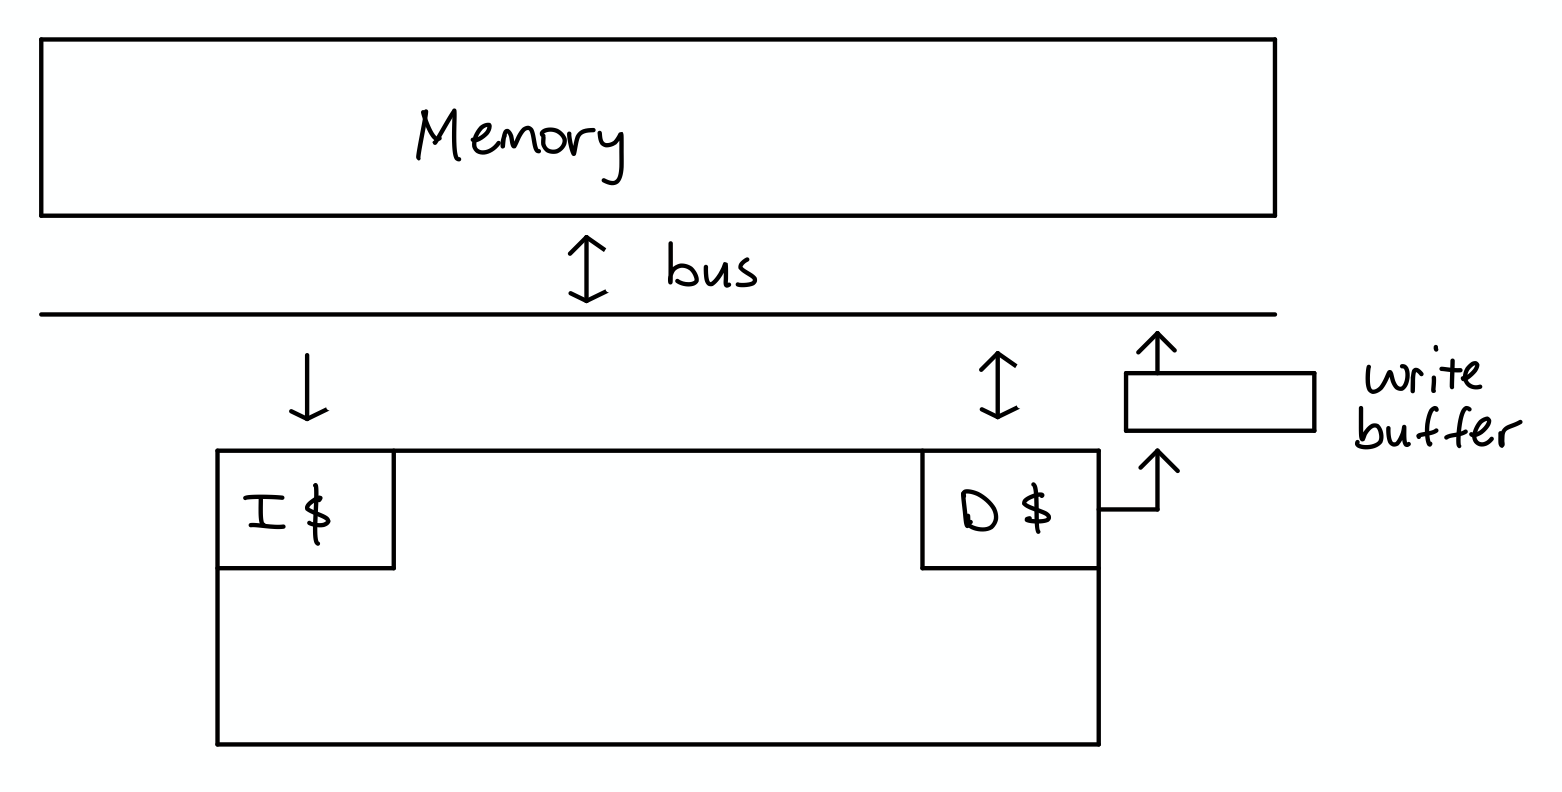
\includegraphics[width=0.65\textwidth]{Screen Shot 2020-05-07 at 00.59.22.png}
        % \caption{}
        % \label{fig:I2Cdemo}
        \end{figure}
    \item What is the purpose of increasing the block size of a cache? What happens if the block size is too large?\par
    \textbf{Increasing the block size reduces compulsory misses (odds of a cold cache are reduced); however, if the block size is too large, this can lead to an increase in conflict misses and an increase in the time to handle a miss.}
    \item Why might one add associativity to a cache? How might one add associativity? Draw a hardware diagram showing how to construct a 2-way set associative cache. What are the drawbacks to set-associative caches?\par
    \textbf{Increasing the associativity reduces conflict misses. Adding more associativity reduces the size of the index and increases the size of the tag because it reduces the number of sets. One adds associativity by using multiple direct-mapped caches with a mux to select between the ways. The drawbacks to associativity are that it increases complexity (a comparator is needed for every cache block in a fully associative cache) and this slows down the cache.}
    \item What is a \textit{split cache} scheme? Why is it beneficial? What might be a disadvantage? Draw a diagram of a single-level, split cache scheme.\par
    \textbf{Split cache scheme splits the data and the instructions into two pipelines. The benefit is that it allows us to read data from both pipelines, however this can exacerbate structural hazards. Split cache scheme is shown below.}
        \begin{figure}[h!]
        \centering
        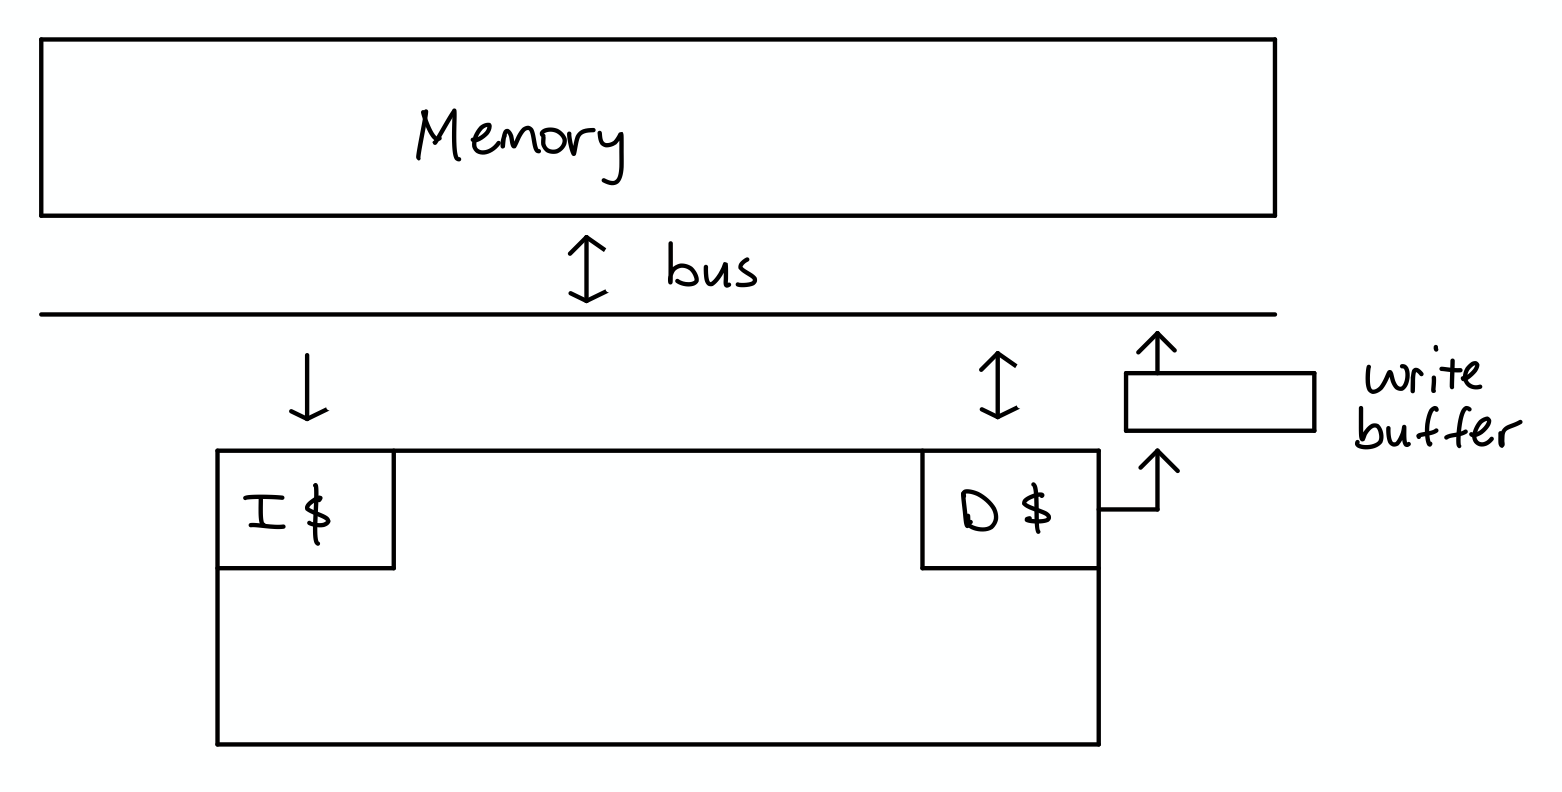
\includegraphics[width=0.65\textwidth]{Screen Shot 2020-05-07 at 00.59.22.png}
        % \caption{}
        % \label{fig:I2Cdemo}
        \end{figure}
    \end{enumerate}
\newpage\item \textbf{(15 points)} For the problem below, a direct-mapped cache is provided the following sequence of \textit{word} addresses: 3, 4, 5, 6, 7, 1, 1, 3, 36, 39, 35, 36.
\begin{enumerate}
    \item Assuming an initially empty, direct-mapped cache with 16 one-word blocks, complete the table below, identifying the tag and index for each word address. Also, indicate whether the access was a hit or miss, and if a it was a miss indicate the type of miss (i.e. compulsory or conflict).
    \begin{table}[ht]
    \centering
    \bgroup
    \def\arraystretch{1.5}
\begin{tabular}{|c|c|c|c|c|c|}
\hline
\textbf{Reference} & \textbf{Address} & \textbf{Tag} & \textbf{Index} & \textbf{Hit/Miss} & \textbf{Type of Miss} \\ \hline
3                  & 00000011         & 0000         & 0011           & Miss              & Compulsory            \\ \hline
4                  & 00000100         & 0000         & 0100           & Miss              & Compulsory            \\ \hline
5                  & 00000101         & 0000         & 0101           & Miss              & Compulsory            \\ \hline
6                  & 00000110         & 0000         & 0110           & Miss              & Compulsory            \\ \hline
7                  & 00000111         & 0000         & 0111           & Miss              & Compulsory            \\ \hline
1                  & 00000001         & 0000         & 0001           & Miss              & Compulsory            \\ \hline
1                  & 00000001         & 0000         & 0001           & Hit               &                       \\ \hline
3                  & 00000011         & 0000         & 0011           & Miss              & Conflict              \\ \hline
36                 & 00100100         & 0010         & 0100           & Miss              & Compulsory            \\ \hline
39                 & 00100111         & 0010         & 0111           & Miss              & Compulsory            \\ \hline
35                 & 00100011         & 0010         & 0011           & Miss              & Compulsory            \\ \hline
36                 & 00100100         & 0010         & 0100           & Miss              & Conflict              \\ \hline
\end{tabular}
\egroup
\end{table}
    \item Calculate the miss rate of the cache above. What is the hit rate?\par
    \textbf{Miss rate $\bm{=\frac{11}{12}=91.7\%}$; Hit rate $\bm{=\frac{1}{12}=8.3\%}$}
    \item Complete the table below assuming a direct-mapped cache with 8 two-word blocks.
\begin{table}[ht]
\centering
\def\arraystretch{1.5}
\begin{tabular}{|c|c|c|c|c|c|c|}
\hline
\textbf{Reference} & \textbf{Address} & \textbf{Tag} & \textbf{Index} & \textbf{Offset} & \textbf{Hit/Miss} & \textbf{Type of Miss} \\ \hline
3                  & 00000011         & 0000         & 001            & 1               & Miss              & Compulsory            \\ \hline
4                  & 00000100         & 0000         & 010            & 0               & Miss              & Compulsory            \\ \hline
5                  & 00000101         & 0000         & 010            & 1               & Hit               &                       \\ \hline
6                  & 00000110         & 0000         & 011            & 0               & Miss              & Compulsory            \\ \hline
7                  & 00000111         & 0000         & 011            & 1               & Hit               &                       \\ \hline
1                  & 00000001         & 0000         & 000            & 1               & Miss              & Compulsory            \\ \hline
1                  & 00000001         & 0000         & 000            & 1               & Hit               &                       \\ \hline
3                  & 00000011         & 0000         & 001            & 1               & Hit               &                       \\ \hline
36                 & 00100100         & 0010         & 010            & 0               & Miss              & Compulsory            \\ \hline
39                 & 00100111         & 0010         & 011            & 1               & Miss              & Compulsory            \\ \hline
35                 & 00100011         & 0010         & 001            & 1               & Miss              & Compulsory            \\ \hline
36                 & 00100100         & 0010         & 010            & 0               & Hit               &                       \\ \hline
\end{tabular}
\end{table}
\item Calculate the miss rate of the cache above. What is the hit rate?\\
\textbf{Miss rate $\bm{=\frac{7}{12}=58.3\%}$; Hit rate $\bm{=\frac{5}{12}=41.7\%}$}
\item Compare the miss rate in part (d) with that of part (b). Does it improve? If so, why?\par
\textbf{Miss rate decreases considerably now because we are using two words to store data. This increases our odds of having a hit.}
\item What two principles make memory caching effective? Be specific in your answer and provide a brief explanation of each principle.\par
\textbf{Two principles that make memory caching effective are temporal locality and spatial locality. Temporal deals with time and states that if a data location is referenced, there is a high likelihood that it will be referenced again. Spatial locality states that if a data location is referenced, there is a high likelihood that nearby locations will be referenced as well.}
\end{enumerate}
\item \textbf{(10 points)} Assuming a direct-mapped cache with a byte-address that is broken up such that bits 0-2 are for the byte offset, bits 3-7 are for the word offset, bits 8-14 are for the index, and bits 15-31 are for the tag, answer the following questions:
\begin{enumerate}
\item How large are the words in this machine?\par
\textbf{$\bm{2^{\mathrm{word\ offset}}=2^5=32}$\ bytes.}
\item How many words are in each cache block? How many bytes are in each cache block?\par
\textbf{$\bm{2^{\mathrm{byte\ offset}}=2^8=256}$\ bytes = 64 words.}
\item How many cache blocks are in the cache? How many sets are in the cache?\par
\textbf{$\bm{2^{\mathrm{index}}=2^{7}=128}$\ blocks. Direct-mapped, therefore 1 block per set = 128 sets.}
\item How large is the data store of this cache?\par
\textbf{128 blocks $\times$ 256 bytes per block = 32768 bytes.}
\item How large is the tag store? Assume a valid and dirty bit are included with each tag.\par
\textbf{$\bm{2^{\mathrm{tag}}=2^{17}=131072}$\ bytes.}
\item If you were to modify the cache to be 2-way set associative but keep the data store the same size, what size would the tag and index be? How large would the tag store be?\par
\textbf{$\bm{2^{\mathrm{index}}=2^{6}=64}$\ blocks; $\bm{2^{\mathrm{tag}}=2^{17}=131072}$\ bytes.}
\item How much memory can the above machine address?\par
\textbf{$\bm{2^{32}=1}$\ MiB.}
\end{enumerate}
\item \textbf{(10 points)} Imagine you have a 1GHz RISC processor with split L1 instruction and data caches, each 32kB in size with a hit time of 1ns. Access to main memory takes 30 ns, and 38\% of instructions access memory. The L1 instruction cache miss rate is 0.7\%, while the L1 data cache miss rate is 6\%.
\begin{enumerate}
\item Calculate the Average Memory Access Time (AMAT) for each of the L1 caches.\par
\textbf{AMAT = Hit time + Miss rate $\bm{\times}$ Miss penalty\\ AMAT = $\bm{1\mathrm{ns} + (0.7\%+6\% \times 30\mathrm{ns})=2.01\mathrm{ms}}$}
    \item Assuming your processor has a CPI of 1.2 with an ideal memory hierarchy, what is the CPI considering memory stalls?\par
    \textbf{}
    \item You are considering the inclusion of a 128kB L2 cache to improve your performance. If the miss rate of the L2 is 3\%, what would the AMAT of the L1 instruction and data caches be with the L2 cache? Assume a 5ns L2 hit time.\par
    \textbf{AMAT = 5ns + (3\% $\bm{\times}$\ 30ns) = 5.9ns}
    \item What would the CPI of your processor be with the L2 cache? What is the speedup due to the L2 cache?\par
    \textbf{}
    \item Why do you suppose the miss rate of the L2 is so much higher than that of the L1?\par
    \textbf{Larger size yields more opportunity for misses.}
    \item Why is the miss rate of the instruction cache lower than the miss rate of the data cache?\par
    \textbf{Instruction cache incorporates lots of spatial and temporal locality compared to data access cache.}
\end{enumerate}
\end{enumerate}
\end{document}